\clearpage
\section{Straddle Attribution and Reconciliation}\label{app:h}\label{app:f}

This appendix explains the straddle account's full-history profit, January 2018--August 2025. It supports the strategy's economic interpretation, not the incremental value of learned sizing or Q allocation.

\subsection{Straddle Profit Attribution}\label{sec:6}

Across 2,599 executed cohorts under learned sizing, options after option charges earned \$1.74 million and stock hedges before hedge costs earned \$1.75 million. Their combined \$3.49 million reconciles to \$3.75 million above cash after the remaining costs, dividends and financing, as shown below.

\begin{figure}[H]\centering
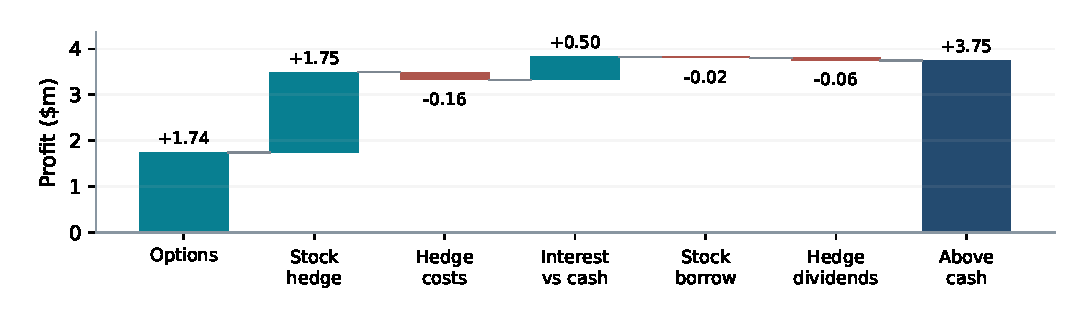
\includegraphics[width=\linewidth]{straddle_bridge.pdf}
\caption{Full-history straddle account, January 2018--August 2025. The option and stock components are read together; the remaining cash flows reconcile them to profit above cash.}\label{fig:straddle-bridge}
\end{figure}

The option and hedge components must be read together. Option marks reflect time decay, stock-price moves and volatility revaluation; the stock position offsets option delta. Positive profits in both components therefore do not establish two independent sources of alpha.

\subsection{Implied and Realized Volatility}\label{sec:7}

Table~\ref{tab:straddle-ivrv-attribution} groups the same cohorts by entry IV versus subsequent RV and completed price path. Combined profit is positive in both path groups when IV exceeds RV and negative when it does not. This is consistent with compensation for selling movement risk. The groups use realized outcomes, so they are descriptive rather than available entry screens.

\begin{table}[H]\centering\small
\caption{Full-history straddle outcomes by completed path and IV versus subsequent RV. Profit combines options after option charges and stock hedges before hedge charges, dividends and financing; totals depend on cohort counts and sizes.}\label{tab:straddle-ivrv-attribution}
\setlength{\tabcolsep}{5pt}\renewcommand{\arraystretch}{1.2}
\begin{tabularx}{\textwidth}{@{}>{\hsize=1.25\hsize\linewidth=\hsize\raggedright\arraybackslash}X>{\hsize=.90\hsize\linewidth=\hsize\raggedright\arraybackslash}X>{\hsize=.75\hsize\linewidth=\hsize\raggedleft\arraybackslash}X>{\hsize=1.10\hsize\linewidth=\hsize\raggedleft\arraybackslash}X@{}}\toprule
\textbf{Price path} & \textbf{IV vs RV} & \textbf{Cohorts} & \textbf{Profit (\$m)}\\\midrule
More persistent & IV < RV & 461 & -4.22\\
More persistent & IV \(\geq\) RV & 846 & +2.93\\
More reversing & IV < RV & 409 & -1.31\\
More reversing & IV \(\geq\) RV & 883 & +6.09\\
\bottomrule\end{tabularx}\end{table}

A more reversing path has absolute entry-to-exit log return no greater than 20\% of the sum of absolute daily log returns; other paths are classified as more persistent. Entry IV is the common annualized European, dividend-escrow volatility that reprices the combined call-and-put entry midpoint premium. Subsequent RV is the square root of 252 times mean squared daily log returns from entry close to actual exit close, without subtracting the sample mean. Three cohorts exited early. The trading signal continues to use ATM-call IV; common straddle IV is an attribution measure only.

The IV--RV relation is not a profit identity: 220 cohorts lose money despite entry IV exceeding subsequent RV. Discrete hedging, jumps, changing gamma and execution charges matter. Classifications also depend on measurement conventions: calendar-time annualization changes 69 classifications, and a dividend adjustment changes six. Positive historical returns alone do not establish alpha after compensation for volatility risk.

\subsection{Accounting Reconciliation}\label{app:attribution-reconciliation}

The 2,599 unique cohorts reconcile to the full-history funded account, including hedge trading costs, stock borrow, dividends and interest above the cash benchmark. One quote-availability convention was inferred; using recovered observed quotes changes aggregate hedge profit by \$367.52. The retained figures use the reconciled saved-account attribution, and this reconstruction difference is not counted as a new profit source. Section~\ref{app:reproduction} states the limits of snapshot-based reproduction.
\FloatBarrier
